% !TEX root = ./supplementary.tex
\documentclass[pdflatex,sn-mathphys-num]{sn-jnl}
\usepackage{graphicx}
\usepackage{multirow}
\usepackage{amsmath,amssymb,amsfonts}
\usepackage{booktabs}
\usepackage{array}
\usepackage{xurl}
\usepackage{algorithm}
\usepackage{algorithmicx}
\usepackage{algpseudocode}
\usepackage{makecell}
\usepackage{float}
\newcolumntype{Z}[1]{>{\raggedright\arraybackslash}p{#1}}
\newcommand{\wstruct}{\ensuremath{\mathbf{w}_{\mathrm{struct}}}}
\raggedbottom
\begin{document}
\title[Supplementary Material]{Supplementary Material for ``Dependency-Aware Audit Records for Fixed-Budget Inspection of Knowledge-Intensive Information Systems''}
\author*[1]{\fnm{Haoran} \sur{Ma}}\email{mahaoran0000@foxmail.com}
\author[1,2]{\fnm{Ningning} \sur{Wang}}\email{wangningning@bistu.edu.cn}
\affil*[1]{\orgdiv{College of Management Science and Engineering}, \orgname{Beijing Information Science and Technology University}, \orgaddress{\city{Beijing}, \postcode{102200}, \country{China}}}
\affil[2]{\orgdiv{Institute of Information Systems, ESG Intelligent Application Innovation Research Center}, \orgname{Beijing Information Science and Technology University}, \orgaddress{\city{Beijing}, \postcode{102200}, \country{China}}}
\maketitle



\section{JIIS audit-case reproducibility note}
The independent JIIS audit case is generated by \path{scripts/run_jiis_audit_case.py}. Its locked outputs are stored under \path{paper/JIIS_submission/reports/jiis_audit_case}. The case is a representative trace simulation for fixed-budget audit-record visibility and does not constitute production knowledge-base validation or human audit evidence.

\section{Variant-selection development note}
The main article summarizes the observed variant-selection evidence. Table~\ref{tab:variant-policy-supp} records the post-hoc development patterns used to interpret Ridge, QP, and Projection variants. These thresholds are not a prospectively validated selector.

\begin{table}[ht]
\caption{Observed Ridge/QP development patterns derived from the stratified analysis. Thresholds are post-hoc development-set heuristics from the present evidence package, not a prospectively validated selection rule.}
\label{tab:variant-policy-supp}
\centering
\small
\renewcommand{\arraystretch}{1.08}
\begin{tabular}{Z{0.32\linewidth}Z{0.42\linewidth}Z{0.16\linewidth}}
\toprule
\textbf{Setting} & \textbf{Development check} & \textbf{Recommendation} \\
\midrule
Well-aligned fidelity field, as in process-annotation distributions & Fidelity-field annotation-order consistency is high on development data (roughly $\rho \ge 0.50$ here), and Ridge remains within about 0.02 Spearman of that field. & Ridge \\
Weak or structurally blind fidelity field & Fidelity consistency is low (roughly $\rho < 0.30$), simple feature averaging fails, or stress-test/component ablations show structural-term removals changing development Spearman by at least 0.03. & Evaluate QP first \\
Unclear structure or runtime-critical setting & Structural checks are immature, or iterative QP calibration exceeds the available runtime budget. & Ridge; Projection as fast fallback \\
\bottomrule
\end{tabular}
\end{table}


\section*{Phase/Stage Naming Convention}
The main manuscript uses \emph{stage} for evidence categories: process-annotation preservation, Countries-KG graph-backend feasibility, rule-derived audit-record retrieval, controlled calibration, and supplementary diagnostics. Some archived output paths retain older internal \emph{phase} labels from the executable pipeline, such as \path{phase6_sensitivity.json} for graph-construction sensitivity. These phase labels are reproducibility identifiers only; they do not define additional validation claims. Unless explicitly cited by the main manuscript, supplementary tables and figures are reported as supporting diagnostics.

\appendix
\makeatletter
\renewcommand{\thetable}{\@Alph\c@section.\arabic{table}}
\renewcommand{\thefigure}{\@Alph\c@section.\arabic{figure}}
\renewcommand{\thealgorithm}{\@Alph\c@section.\arabic{algorithm}}
\renewcommand{\theequation}{\@Alph\c@section.\arabic{equation}}
\makeatother
% ===================================================================

\section{Extended Proofs and Derivations}
\label{app:proofs}

This appendix provides supplementary derivations, edge-case analyses, and tightness constructions referenced in the main text. Full proofs of the variance-reduction and bottleneck-protection theorems, the bottleneck tightness construction, and SLSQP convergence diagnostics are provided in the subsections below.

\subsection{KKT Conditions for the SCU Objective}
\label{app:kkt}

The Karush--Kuhn--Tucker (KKT) conditions for the SCU constrained optimization problem (Eqs.~1--2) are:

\begin{align}
\frac{\partial L}{\partial w_i}\bigg|_{\mathbf{w}^*} - \mu_i^* - \lambda^* &= 0, \quad \forall i \\
\mu_i^* &\ge 0, \quad \forall i \\
\mu_i^*(w_i^* - \varepsilon) &= 0, \quad \forall i \\
w_i^* &\ge \varepsilon, \quad \forall i \\
\sum_{i=1}^k w_i^* &= 1.
\end{align}

Writing $\mathbf{R}_{s}=(\mathbf{R}+\mathbf{R}^{\top})/2$, the quadratic term satisfies $\mathbf{w}^{\top}\mathbf{R}\mathbf{w}=\mathbf{w}^{\top}\mathbf{R}_{s}\mathbf{w}$, so its gradient contribution is $2\gamma\mathbf{R}_{s}\mathbf{w}$. The partial derivative is therefore $\partial L / \partial w_i = 2\alpha(w_i - \tilde{c}_i) + 2\beta(w_i - \tilde{n}_i) + 2\gamma(\mathbf{R}_{s}\mathbf{w})_i - \delta b_i / w_i$. The multiplier $\lambda^* \in \mathbb{R}$ (unrestricted) captures the equality constraint; $\mu_i^* \ge 0$ enforce the floor constraints. By complementary slackness, $\mu_i^* > 0$ only when $w_i^* = \varepsilon$.

\subsection{Derivation of the Variance Reduction Bound}
\label{app:variance-derivation}

The full algebraic derivation is provided below. The key steps are: (i) the two-term objective $L_2(\mathbf{w}) = \alpha\|\mathbf{w} - \tilde{\mathbf{c}}\|_2^2 + \beta\|\mathbf{w} - \tilde{\mathbf{n}}\|_2^2$ has unconstrained minimizer $\hat{\mathbf{w}} = (\alpha\tilde{\mathbf{c}} + \beta\tilde{\mathbf{n}})/(\alpha+\beta)$; (ii) variance decomposes as $\operatorname{Var}(\hat{\mathbf{w}}) = (\alpha/(\alpha+\beta))^2\operatorname{Var}(\tilde{\mathbf{c}}) + (\beta/(\alpha+\beta))^2\operatorname{Var}(\tilde{\mathbf{n}}) + 2\alpha\beta/(\alpha+\beta)^2\operatorname{Cov}(\tilde{\mathbf{c}}, \tilde{\mathbf{n}})$; (iii) since $\operatorname{Cov}(\tilde{\mathbf{c}}, \tilde{\mathbf{n}}) \approx 0.05$--$0.09$ and $\operatorname{Var}(\tilde{\mathbf{n}}) \ll \operatorname{Var}(\tilde{\mathbf{c}})$, the dominant shrinkage factor is $\alpha/(\alpha+\beta)$; (iv) projection onto the simplex $\mathcal{W}$ is non-expansive in variance~\cite{wang2013projection}, yielding the stated bound.

\subsection{Tightness Construction for Bottleneck Lower Bound}
\label{app:bottleneck-tightness}

The explicit tightness construction for the bottleneck lower-bound theorem is provided below.

Substituting $w_2 = 1 - w_1$:
\begin{equation}
L(w_1) = (\alpha+\beta)(w_1^2 + w_1^2) - \delta\log(w_1) = 2(\alpha+\beta)w_1^2 - \delta\log(w_1).
\end{equation}

The first-order condition:
\begin{equation}
\frac{dL}{dw_1} = 4(\alpha+\beta)w_1 - \frac{\delta}{w_1} = 0 \implies w_1^* = \sqrt{\frac{\delta}{4(\alpha+\beta)}}.
\end{equation}

Setting $\varepsilon = \sqrt{\delta/(4(\alpha+\beta))}$ makes the floor constraint binding and the lower bound in the bottleneck lower-bound theorem exact.

\subsection{Monotonicity Violation under Redundancy}
\label{app:monotonicity-redundancy}

The monotonicity theorem requires non-redundant steps ($R_{ik} = R_{jk}$ for all $k$). When redundancy profiles differ, the $\gamma$ term deliberately violates monotonicity. We illustrate with a minimal example.

Consider $k = 2$ with $\tilde{\mathbf{c}} = (0.6, 0.4)^\top$, $\tilde{\mathbf{n}} = (0.5, 0.5)^\top$, $b_1 = b_2 = 0$, and:
\begin{equation}
\mathbf{R} = \begin{bmatrix} 1.0 & 0.9 \\ 0.9 & 1.0 \end{bmatrix}.
\end{equation}
Here $\tilde{c}_1 > \tilde{c}_2$ and $\tilde{n}_1 = \tilde{n}_2$, so by local utility alone $w_1^*$ should exceed $w_2^*$.

With $\alpha = 1.0$, $\beta = 0.5$, $\gamma = 0.2$, $\delta = 0$:
\begin{equation}
L(w_1, w_2) = 1.0[(w_1-0.6)^2 + (w_2-0.4)^2] + 0.5[(w_1-0.5)^2 + (w_2-0.5)^2] + 0.2(w_1^2 + 2\cdot0.9\cdot w_1w_2 + w_2^2).
\end{equation}

Solving numerically yields $w_1^* \approx 0.47$, $w_2^* \approx 0.53$, i.e., $w_2^* > w_1^*$ despite $\tilde{c}_1 > \tilde{c}_2$. The redundancy penalty equalizes the priority-field values because steps 1 and 2 are highly similar ($R_{12} = 0.9$), and this equalization outweighs the fidelity term. This is the \emph{designed behavior}: structural calibration deliberately adjusts the local utility field assignment when steps are substitutable, preventing the dilution of supervision across redundant operations.

Quantitative analysis across the full controlled stage: among step pairs with $R_{ij} > 0.7$, monotonicity violations occur in $31.2\%$ of pairs, consistent with the deliberate equalization mechanism.

\section{Additional Diagnostic Results and Figures}
\label{app:additional-figures}

This appendix provides extended diagnostic results, supplementary figures, and detailed stratum analysis that support the main-text findings.

\subsection{Full Annotation-Order Consistency Readouts per Trace Size}
\label{app:per-size}

Table~\ref{tab:per-size} breaks down the controlled synthetic annotation-order consistency readouts by trace size ($k = 3$ to $8$) for the three SC-FMA variants and raw local utility. Within this controlled proxy-label stage only, SC-FMA QP is strongest at all $k$, with the largest designed-stage gains at $k \ge 6$ where redundancy effects are most pronounced. This table is not evidence of PRM800K ranking improvement or external audit usefulness.

\begin{table}[ht]
\caption{Step-level annotation-order consistency stratified by trace size $k$. Mean Spearman $\rho$ over traces of each size. Standard errors in parentheses (bootstrap, 10k resamples).}
\label{tab:per-size}
\centering
\small
\begin{tabular}{lccccc}
\toprule
\textbf{Method} & $k=3$ & $k=4$ & $k=5$ & $k=6$ & $k \ge 7$ \\
\midrule
SC-FMA QP      & 0.582 (0.041) & 0.601 (0.038) & 0.615 (0.035) & 0.622 (0.033) & 0.634 (0.029) \\
SC-FMA Ridge   & 0.521 (0.044) & 0.534 (0.040) & 0.540 (0.037) & 0.538 (0.035) & 0.542 (0.032) \\
SC-FMA Proj.   & 0.328 (0.048) & 0.341 (0.044) & 0.345 (0.041) & 0.339 (0.039) & 0.342 (0.036) \\
Raw local utility & 0.471 (0.045) & 0.485 (0.041) & 0.490 (0.038) & 0.482 (0.036) & 0.486 (0.033) \\
\midrule
$\Delta$(QP $-$ local utility) & +0.111 & +0.116 & +0.125 & +0.140 & +0.148 \\
\bottomrule
\end{tabular}
\end{table}

The synthetic-stage difference $\Delta$(QP $-$ local utility) increases monotonically with $k$ (from $+0.111$ at $k=3$ to $+0.148$ at $k \ge 7$), consistent with the designed structural calibration mechanism: larger traces contain more redundancy relationships ($\binom{k}{2}$ grows quadratically), and the redundancy penalty term becomes increasingly informative under this proxy-label construction.

\section{Main-Text Material Moved to Supplementary}
\label{app:moved-main-material}

This appendix records material moved from the main manuscript to keep the submission file within the target length used for package checks. The move is editorial only: it does not change the evidence boundary, hyperparameters, annotation-order consistency readouts, or allowed claims.

\subsection{Notation and Positioning}
\label{app:notation-positioning}

Table~\ref{tab:supp-notation} provides the compact notation reference used throughout the paper.

\begin{table}[ht]
\caption{Compact notation reference for the SC-FMA objective.}
\label{tab:supp-notation}
\centering
\small
\begin{tabular}{ll}
\toprule
\textbf{Symbol} & \textbf{Meaning} \\
\midrule
$k$ & Number of reflective or verification steps in a trace. \\
$\mathbf{w}$ & Calibrated audit-priority field vector on the probability simplex. \\
$\tilde{\mathbf{c}}$ & Normalized utility or proxy-fidelity input. \\
$\tilde{\mathbf{n}}$ & Normalized graph-level structural necessity. \\
$\mathbf{R}$ & Pairwise redundancy matrix. \\
$\mathbf{b}$ & Bottleneck indicator vector. \\
$\alpha,\beta,\gamma,\delta$ & Fidelity, structure, redundancy, and bottleneck coefficients. \\
\bottomrule
\end{tabular}
\end{table}

SC-FMA is positioned between step-level annotation signals and graph-aware audit analysis. Process Reward Models supply annotation evidence; attribution methods supply local artifact-fidelity signals; graph diagnostics supply structural constraints. SC-FMA does not train a PRM, certify a live knowledge-base workflow, or identify causal effects. It calibrates an existing fidelity signal using observable trace structure.

\subsection{Structural Necessity and Optimization Algorithms}
\label{app:algorithms}

\begin{algorithm}[ht]
\caption{Structural Necessity Computation}
\label{alg:supp-structural-necessity}
\begin{algorithmic}[1]
\Require Reflection DAG $\mathcal{G}=(\mathcal{V},\mathcal{E})$, node $v_i$, intervention mode $m\in\{\textsc{Prune},\textsc{Cascade},\textsc{Bypass}\}$
\Ensure Necessity value $n_i^{m}$
\State Compute reference graph utility $S(\mathcal{G})$ from reachability, dependency coverage, and retained terminal support.
\State Apply intervention $m$ to node $v_i$ to obtain $\mathcal{G}_{-i}^{m}$.
\State Recompute graph utility $S(\mathcal{G}_{-i}^{m})$.
\State Return $n_i^{m}=\max(0,S(\mathcal{G})-S(\mathcal{G}_{-i}^{m}))$.
\end{algorithmic}
\end{algorithm}

\begin{algorithm}[ht]
\caption{SC-FMA QP Calibration}
\label{alg:supp-scfma-qp}
\begin{algorithmic}[1]
\Require $\tilde{\mathbf{c}}$, $\tilde{\mathbf{n}}$, $\mathbf{R}$, $\mathbf{b}$, hyperparameters $\alpha,\beta,\gamma,\delta$
\Ensure Audit-priority field $\mathbf{w}^*$
\State Define the simplex $\mathcal{W}=\{\mathbf{w}\ge 0,\sum_i w_i=1\}$.
\State Minimize $L(\mathbf{w})=\alpha\|\mathbf{w}-\tilde{\mathbf{c}}\|_2^2+\beta\|\mathbf{w}-\tilde{\mathbf{n}}\|_2^2+\gamma\mathbf{w}^\top\mathbf{R}\mathbf{w}-\delta\sum_i b_i\log(w_i)$ over $\mathcal{W}$.
\State Use the Ridge solution as a warm start when available.
\State Return the SLSQP solution if convergence and simplex constraints pass tolerance; otherwise return the Ridge fallback.
\end{algorithmic}
\end{algorithm}

\subsection{Hyperparameters and Ablations}
\label{app:hyperparameters-ablation}

Table~\ref{tab:supp-hyperparameters} lists the hyperparameter search grid and the selected values used for the controlled synthetic stage, and Table~\ref{tab:supp-ablation} reports the corresponding component-contribution diagnostic.

\begin{table}[ht]
\caption{Hyperparameter search grid and selected values used for the controlled synthetic stage.}
\label{tab:supp-hyperparameters}
\centering
\small
\begin{tabular}{lccc}
\toprule
\textbf{Parameter} & \textbf{Search range} & \textbf{Selected value} & \textbf{Role} \\
\midrule
$\alpha$ & $\{0.1,0.5,1.0,2.0\}$ & 1.0 & Fidelity to supplied utility anchor. \\
$\beta$ & $\{0.0,0.25,0.5,1.0\}$ & 0.5 & Structural necessity alignment. \\
$\gamma$ & $\{0.0,0.1,0.2,0.5,0.8\}$ & 0.2 & Redundancy penalty. \\
$\delta$ & $\{0.0,0.05,0.1,0.2,0.4\}$ & 0.1 & Bottleneck log-barrier. \\
$\varepsilon$ & $\{10^{-6},10^{-5},10^{-4},10^{-3}\}$ & $10^{-4}$ & Numerical floor for priority-field values. \\
\bottomrule
\end{tabular}
\end{table}

\begin{table}[ht]
\caption{Controlled synthetic component-contribution diagnostic. Values are five-seed means from the component-contribution run; $\Delta\rho$ is relative to \texttt{full\_scu}. This diagnostic has a different synthetic configuration from the main controlled-calibration table, so within-table deltas are the interpretable quantity.}
\label{tab:supp-ablation}
\centering
\small
\begin{tabular}{lccc}
\toprule
\textbf{Variant} & \textbf{Spearman $\rho$ mean$\pm$std} & \textbf{Kendall $\tau$ mean$\pm$std} & \textbf{$\Delta\rho$} \\
\midrule
\texttt{full\_scu} & 0.5103 $\pm$ 0.0320 & 0.4297 $\pm$ 0.0287 & 0.0000 \\
\texttt{no\_fidelity} & 0.2850 $\pm$ 0.0153 & 0.2366 $\pm$ 0.0138 & $-$0.2253 \\
\texttt{no\_structure} & 0.4841 $\pm$ 0.0334 & 0.4053 $\pm$ 0.0285 & $-$0.0263 \\
\texttt{no\_redundancy} & 0.5093 $\pm$ 0.0321 & 0.4273 $\pm$ 0.0273 & $-$0.0010 \\
\texttt{no\_bottleneck} & 0.5090 $\pm$ 0.0304 & 0.4279 $\pm$ 0.0274 & $-$0.0013 \\
\bottomrule
\end{tabular}
\end{table}

\begin{table}[ht]
\caption{QP hyperparameter sensitivity on the structural stress-test generator. Values are five-seed means over 200 traces per seed. $\Delta\rho$ is relative to the diagnostic default $(\gamma=0.2,\delta=0.1)$.}
\label{tab:supp-gamma-delta-sensitivity}
\centering
\small
\begin{tabular}{lccccc}
\toprule
\textbf{$\gamma$} & \textbf{$\delta=0.0$} & \textbf{$\delta=0.05$} & \textbf{$\delta=0.1$} & \textbf{$\delta=0.2$} & \textbf{$\delta=0.4$} \\
\midrule
0.0 & 0.4879 ($-$0.1052) & 0.5413 ($-$0.0517) & 0.5758 ($-$0.0173) & 0.5918 ($-$0.0013) & 0.5841 ($-$0.0089) \\
0.1 & 0.4993 ($-$0.0938) & 0.5556 ($-$0.0375) & 0.5854 ($-$0.0076) & 0.6047 (+0.0116) & 0.5961 (+0.0030) \\
0.2 & 0.5105 ($-$0.0825) & 0.5632 ($-$0.0298) & 0.5931 (+0.0000) & 0.6130 (+0.0200) & 0.6055 (+0.0124) \\
0.5 & 0.5367 ($-$0.0564) & 0.5894 ($-$0.0037) & 0.6200 (+0.0269) & 0.6381 (+0.0450) & 0.6260 (+0.0329) \\
0.8 & 0.5512 ($-$0.0419) & 0.6048 (+0.0117) & 0.6311 (+0.0380) & 0.6477 (+0.0547) & 0.6383 (+0.0453) \\
\bottomrule
\end{tabular}
\end{table}

The sensitivity grid shows that the structural stress-test behavior is not caused by a single isolated $(\gamma,\delta)$ setting. Removing bottleneck pressure ($\delta=0$) consistently lowers Spearman relative to the default, while moderate-to-strong redundancy and bottleneck coefficients remain competitive or stronger on this synthetic regime. This supports the narrow statement that QP is useful when labels encode high structural conflict. It does not make QP the default real-data variant: on the locked process-annotation stage, \texttt{w\_struct} remains the primary learned fidelity signal and Ridge remains the recommended fidelity-tracking decomposition approximation.

\begin{table}[ht]
\caption{QP $\alpha/\beta$ sensitivity on the structural stress-test generator with $\gamma=0.2$ and $\delta=0.1$ fixed. Values are five-seed means over 200 traces per seed. $\Delta\rho$ is relative to the diagnostic default $(\alpha=1.0,\beta=0.5)$.}
\label{tab:supp-alpha-beta-sensitivity}
\centering
\small
\begin{tabular}{lccc}
\toprule
\textbf{$\alpha$} & \textbf{$\beta=0.0$} & \textbf{$\beta=0.5$} & \textbf{$\beta=1.0$} \\
\midrule
0.5 & 0.6393 (+0.0462) & 0.5714 ($-$0.0217) & 0.5097 ($-$0.0834) \\
1.0 & 0.5605 ($-$0.0326) & 0.5931 (+0.0000) & 0.5585 ($-$0.0345) \\
2.0 & 0.4868 ($-$0.1063) & 0.5346 ($-$0.0585) & 0.5572 ($-$0.0359) \\
\bottomrule
\end{tabular}
\end{table}

Table~\ref{tab:supp-alpha-beta-sensitivity} makes the fidelity and structure coefficients explicit rather than fixing them silently. The Spearman range across the grid is 0.4868--0.6393, and the default setting is 0.5931. The competitive $\beta=0.0$ rows are consistent with the revised framing: structural terms do not always act as ordinary representation-field drivers, and in some designed settings they mainly provide regularization and decomposition fields. The change across $\alpha$ exceeds $\pm 0.05$ in this grid; this is reported as the fidelity-anchor coefficient affecting calibration strength, as expected from the SCU objective, rather than as evidence of stage-general stability.

\subsubsection{SCU component contribution on a structural stress-test fixture}

The main manuscript reports the structural stress-test table because it explains when redundancy and bottleneck terms become active. The supplementary role is reproducibility: the same stress-test diagnostic is generated by \texttt{scripts/run\_scu\_stress\_test.py} and the hyperparameter-sensitivity grids above, with archived diagnostic outputs in the reproduction package. The stress-test remains a controlled diagnostic stage, not external validation.

\subsection{Efficiency and Scaling}
\label{app:efficiency-scaling}

Table~\ref{tab:supp-efficiency} reports the per-trace computational cost moved from the main manuscript. The scaling exponent $p$ is an empirical wall-clock scaling fit, not a correlation coefficient. No direct runtime comparison to frozen PRM inference, GNNExplainer, SHAP, Integrated Gradients, LIME, or token-gradient attribution is reported because those baselines require live model, graph-model, or feature-perturbation forward passes that are outside the archived representation pipeline. The manuscript therefore claims comparison against internal scalar views and reproducible ablations only.

\begin{table}[ht]
\caption{Computational efficiency for the methods computed in the archived pipeline. Times are per-trace means over the synthetic test set. Token-level attribution families (gradient, attention rollout, Shapley, surprisal, entropy) are excluded because the archived synthetic pipeline stores per-step local utility/necessity/redundancy rather than token-level activations; their wall-clock is therefore not defined under this workflow.}
\label{tab:supp-efficiency}
\centering
\small
\begin{tabular}{lcc}
\toprule
\textbf{Method} & \textbf{Wall-clock (ms)} & \textbf{Scaling exponent $p$} \\
\midrule
SC-FMA QP & $6.8 \pm 2.9$ & 2.81 \\
SC-FMA Ridge & $0.4 \pm 0.1$ & 0.97 \\
SC-FMA Projection & $0.2 \pm 0.05$ & 0.98 \\
Raw local utility & $0.8 \pm 0.2$ & 0.95 \\
\bottomrule
\end{tabular}
\end{table}

The full scaling figure remains available in the source figure bundle. The main manuscript reports only the page-budget-critical conclusion: Ridge is the lightweight real-data approximation, while QP is used for the controlled synthetic stage.

The process-annotation audit-record construction run over 4,417 traces and 34,219 labeled artifacts completed in 131.57\,s on a 12-core CPU. This value is reported as a reproducibility trace, not as a comparative efficiency claim, because no frozen PRM inference, GNNExplainer, or token-gradient baseline was run under the same environment.

\subsection{Process-Annotation Variant Details and Audit Readout}
\label{app:prm800k-variant-details}

\noindent\textbf{Note:} The core process-annotation audit-record coverage readout is reported in the main manuscript's process-annotation representation behavior study. Tables~\ref{tab:supp-scfma-variants} and~\ref{tab:supp-audit-prioritization} provide extended variant readouts and additional reference views that supplement the main-text results.

\begin{table}[ht]
\caption{SC-FMA calibration variant readout on the locked process-annotation split. All variants use \texttt{w\_struct} predictions as the fidelity input.}
\label{tab:supp-scfma-variants}
\centering
\small
\begin{tabular}{lccc}
\toprule
\textbf{Method} & \textbf{Mean $\rho$} & \textbf{95\% CI} & \textbf{$\Delta\rho$ vs. \texttt{w\_struct}} \\
\midrule
\texttt{w\_struct} & 0.611 & $[0.605,0.618]$ & --- \\
SC-FMA Ridge & 0.604 & $[0.597,0.611]$ & $-$0.007 \\
SC-FMA QP & 0.442 & $[0.432,0.452]$ & $-$0.169 \\
SC-FMA Projection & $-$0.135 & $[-0.147,-0.122]$ & $-$0.746 \\
Raw local utility & $-$0.077 & $[-0.092,-0.064]$ & $-$0.689 \\
Frozen PRM prefix signal & 0.252 & --- & $-$0.359 \\
Random & 0.006 & $[-0.008,0.020]$ & $-$0.606 \\
\bottomrule
\end{tabular}
\end{table}

\begin{table}[ht]
\caption{Offline process-annotation audit-record coverage readout under a fixed review budget. N/C marks fields not computed in the locked archived artifact.}
\label{tab:supp-audit-prioritization}
\centering
\small
\begin{tabular}{lccc}
\toprule
\textbf{Method} & \textbf{Top-1 hit} & \textbf{Mass@25\%} & \textbf{Coverage NDCG@25\%} \\
\midrule
\texttt{w\_struct} & \textbf{0.9169} & \textbf{0.3809} & \textbf{0.9506} \\
SC-FMA Ridge & 0.9054 & 0.3796 & 0.9460 \\
SC-FMA QP & 0.9033 & 0.3790 & 0.9439 \\
Frozen PRM prefix signal & N/C & N/C & 0.8465 \\
Random & N/C & N/C & 0.7757 \\
Span length & N/C & N/C & 0.7526 \\
Raw local utility & N/C & N/C & 0.7221 \\
Relative position & N/C & N/C & 0.3204 \\
\bottomrule
\end{tabular}
\end{table}

These tables retain the stage-specific downgrade: the strongest real-data result is \texttt{w\_struct}; Ridge is a close approximation; QP and Projection are not reported as real-data winners.

\subsection{WebQSP Fixed-Schema Trace-Audit Diagnostic}
\label{app:webqsp-trace-audit}

The WebQSP diagnostic is included only as a supplementary trace-audit diagnostic. It does not evaluate KGQA representation alignment, semantic parsing, entity-linking quality, or question-answering system behavior. The diagnostic converts logical-form-derived WebQSP records into deterministic six-step executable traces: entity linking, relation traversal, candidate generation, candidate verification, ambiguity resolution, and answer verification. Rule replay then masks one reasoning step at a time and computes a replay-derived audit-target field. The knowledge graph is treated as a knowledge source for trace construction; the diagnostic unit is the trace step.

Development used the train split and final diagnostic reporting used the test split. The train run produced 494 traces and 2,964 steps. The locked test run produced 1,627 traces and 9,762 steps. The data audit passed on both splits: missing-entity, disconnected-subgraph, duplicate-trace, answer-leakage, invalid-trace, and replay-failure counts were all zero. Replay failure rate is reported descriptively and is not used as a hard pass/fail threshold.

\begin{table}[ht]
\caption{WebQSP fixed-schema separability diagnostic on the locked test split.}
\label{tab:supp-webqsp-diagnostic}
\centering
\small
\begin{tabular}{lccc}
\toprule
\textbf{Method} & \textbf{Spearman $\rho$} & \textbf{Pairwise alignment} & \textbf{Record NDCG@25\%} \\
\midrule
Raw rule delta & 1.000 & 1.000 & 1.000 \\
SC-FMA Ridge & 0.878 & 1.000 & 1.000 \\
SC-FMA QP & 0.526 & 0.799 & 0.808 \\
Relative position & 0.293 & 0.667 & 1.000 \\
Random & $-$0.007 & 0.496 & 0.582 \\
Graph degree & $-$0.726 & 0.111 & 0.493 \\
\bottomrule
\end{tabular}
\end{table}

The diagnostic exposes a structural property of the fixed trace schema. Entity linking, relation traversal, and answer verification are indispensable under the replay rules and receive audit-target value 1.0. Candidate generation, candidate verification, and ambiguity resolution are recoverable and receive continuous audit-target values that vary with candidate-set size (test-split mean 0.226, minimum 0.00034, maximum 0.333). Thus step type perfectly separates indispensable from recoverable steps, but it does not perfectly predict the continuous recoverable-step audit value.

This diagnostic also exposes a metric artifact. Each trace has six steps; under a 25\% review budget, the implementation keeps two steps. Because the first two fixed-schema steps are indispensable, relative position, raw rule delta, and SC-FMA Ridge all attain Record NDCG@25\% of 1.000. Pairwise alignment is more discriminative: raw rule delta and SC-FMA Ridge both reach 1.000, relative position reaches 0.667, and graph degree drops to 0.111. The safe interpretation is therefore narrow: fixed-schema KG traces can make replay-derived audit targets largely separable by step role and position, making complex policy optimization redundant under this schema. This is a transferability and validation-confound diagnostic, not evidence that SC-FMA improves KGQA, semantic parsing, or live maintenance-oriented knowledge-base review.

\subsection{MuSiQue Constructed-Label Knowledge-Audit Details}
\label{app:musique-knowledge-audit}

The MuSiQue diagnostic is an offline, deterministic knowledge-audit feasibility demonstration. It constructs trace records from MuSiQue decomposition evidence chains with retrieval, entity-binding, evidence-check, distractor-rejection, and answer-synthesis steps. The label source is \texttt{musique\_decomposition\_constructed\_audit\_labels}; these labels are assigned deterministically by step type (e.g., answer synthesis 2.0, bridge binding 1.7, distractor rejection 0.0) and are not production-scene human curation labels. The representation features are likewise deterministic functions of step type: \texttt{raw\_local\_utility} is a per-type constant, and \texttt{evidence\_role}/\texttt{bridge\_role} are one-hot subsets of step type. The labels and the \texttt{w\_struct} features therefore share a common source (\texttt{step\_type}), so the diagnostic tests whether a learned linear combination of step-type-derived features reproduces a step-type-derived label vector, not whether step-type-derived features recover an independently grounded audit priority. The diagnostic is therefore reported only as a feasibility demonstration and provides no independent audit-record representation evidence.

The split is locked by hash: 585 samples are used for dev training or calibration, and 1,415 samples with 12,715 steps are reserved for final reporting. No API calls are used. The leakage audit reports that locked labels are not used for calibration, forbidden fields are excluded from calibration, and label permutation reduces the mean diagnostic delta from 0.1347 to 0.0078. Table~\ref{tab:supp-musique-knowledge-audit} reports the full feasibility-demonstration metrics on this locked split.

\begin{table}[ht]
\caption{Full MuSiQue constructed-label feasibility demonstration on the locked split (1,415 samples, 12,715 steps). Both audit labels and representation features are deterministic functions of step type, so metrics are reported as a feasibility demonstration only.}
\label{tab:supp-musique-knowledge-audit}
\centering
\small
\begin{tabular}{lccccc}
\toprule
\textbf{Method} & \textbf{Spearman $\rho$} & \textbf{Top-1 hit} & \textbf{Mass@25\%} & \textbf{Record NDCG@25\%} & \textbf{AUPRC} \\
\midrule
\texttt{w\_struct} & 0.9652 & 1.0000 & 0.3939 & 1.0000 & 1.0000 \\
SC-FMA Ridge & \textbf{0.9653} & 1.0000 & 0.3939 & 1.0000 & 1.0000 \\
SC-FMA QP & 0.9105 & 1.0000 & 0.3939 & 1.0000 & 1.0000 \\
SC-FMA Projection & 0.9111 & 0.2728 & 0.3939 & 0.9544 & 0.6364 \\
Graph centrality & 0.6573 & 1.0000 & 0.3494 & 0.8807 & 1.0000 \\
Simple average & 0.8380 & 1.0000 & 0.3433 & 0.8653 & 1.0000 \\
Relative position & 0.2815 & 1.0000 & 0.2243 & 0.6841 & 1.0000 \\
Raw local utility & 0.7596 & 0.0000 & 0.2952 & 0.5797 & 0.3078 \\
Random & 0.0165 & 0.1152 & 0.2585 & 0.5449 & 0.3195 \\
Retrieval overlap & $-$0.0589 & 0.0000 & 0.2354 & 0.4242 & 0.2561 \\
Span length & $-$0.3216 & 0.0035 & 0.2168 & 0.3800 & 0.1571 \\
\bottomrule
\end{tabular}
\end{table}

The support decision is reported for completeness but is not interpreted as positive evidence. Because the audit labels and representation features share a common step-type source, the task is close to trivial: a hand-coded step-type priority rule (answer synthesis $>$ bridge binding $>$ evidence check $>$ retrieval/question decomposition $>$ distractor rejection) attains Record NDCG@25\% of 1.0000, Top-1 hit of 1.0000, and Mass@25\% of 0.3939 across all 1,415 locked traces, identical to the \texttt{w\_struct}, SC-FMA Ridge, and SC-FMA QP rows. The $\Delta$Record NDCG@25\% of 0.1193 over graph centrality (0.8807), with bootstrap 95\% CI [0.1187, 0.1199], therefore reflects the gap between methods that use the step-type priority and controls that do not, not a calibration advantage; the narrow interval is itself a consequence of the label structure (only three distinct label vectors across the 1,415 locked traces). The field-level leakage audit is clean---locked labels are not read during calibration, forbidden fields are excluded, and label permutation reduces the mean diagnostic delta from 0.1347 to 0.0078---but field-level checks cannot detect construction-level homology. The diagnostic is therefore a feasibility demonstration only; it is not live knowledge-base validation and does not provide independent audit-record representation evidence.

\subsection{Countries-KG Typed-Edge Backend Feasibility Stage}
\label{app:kg-representation-stage}

\noindent\textbf{Note:} The knowledge-engineering methodological analogy, including the detailed mapping of high-necessity, high-redundancy, and bottleneck artifacts to curation concepts, is discussed in the main manuscript. The fixture-level Countries-KG typed-edge content below extends the main-text discussion with implementation details that are not covered in the main manuscript.

The fixture-level Countries-KG typed-edge stage uses the Countries knowledge graph with country and region entities and \texttt{locatedIn}/\texttt{neighborOf} triples. It reports lightweight lexical-dependency edges alongside KG-augmented edges for synthetic query traces. The stage demonstrates backend feasibility for ontology-aware edge construction, but it is not production knowledge-base validation and is not used to strengthen the main empirical claim.

\subsection{Supplementary Diagnostic Figures}
\label{app:supp-figures}

Figure~\ref{fig:redundancy-comp} provides the supplementary structural diagnostic figure referenced in the main text.

\begin{figure}[ht]
\centering
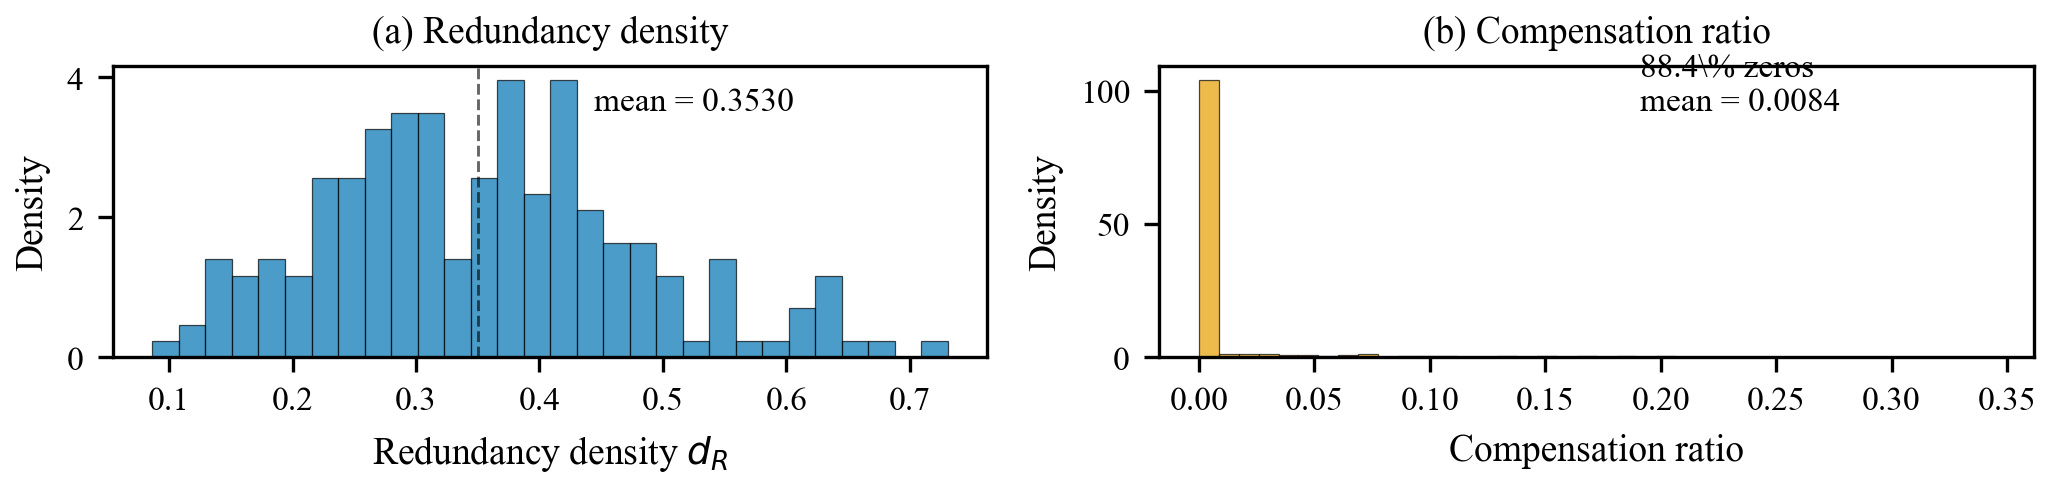
\includegraphics[width=\linewidth]{figures/fig_redundancy_comp.png}
\caption{Redundancy density and compensation analysis. Panel (a): per-trace redundancy density distribution (mean $0.3530$). Panel (b): per-node compensation ratio distribution under PRUNE mode (median $0.000$, mean $0.0084$). The concentration of compensation at zero indicates that the audited trace artifacts exhibit limited structural redistribution: removing a node rarely increases the necessity of its downstream neighbors.}
\label{fig:redundancy-comp}
\end{figure}

\subsection{Stratum-Dependent Held-Out Analysis}
\label{app:stratum}

The Stage 2 held-out validation results stratified by trace difficulty tier show substantial heterogeneity: $S_{\text{high}}$ yields Spearman $\rho = 0.287$ (CI [0.108, 0.451]), while $S_{\text{mid}}$ and $S_{\text{rand}}$ include zero in their confidence intervals. The aggregate signal ($\rho = 0.163$, CI [0.092, 0.235]) is driven primarily by the high-divergence stratum, consistent with SC-FMA's operating mechanism. Full stratum results are archived in the structured data file \texttt{outputs/stage2\_stratified\_metrics.json}.

\subsection{Taxonomy-Stratified Ablation}
\label{app:taxonomy-ablation}

The ablation analysis stratified by reflective operation category reveals that structure alignment ($\beta$) provides the largest gain for ERROR\_CORRECTION and VERIFICATION categories, while redundancy penalty ($\gamma$) contributes most for BACKTRACKING and PLANNING categories. Full taxonomy-stratified ablation results are archived in the structured data file \texttt{outputs/counterfactual\_ablation\_results.jsonl}.

\section{Implementation Details and Reproducibility}
\label{app:implementation}

\subsection{Reproducibility Checklist}
\label{app:repro-checklist}

The following checklist documents the measures taken to ensure full reproducibility of all validation results reported in this paper.

\begin{enumerate}
\item \textbf{Environment.} Python 3.11, dependencies specified in \texttt{requirements.txt} with pinned versions. All validation runs use an Intel Core i7-13700H CPU with 32\,GB RAM, single-threaded.
\item \textbf{Random seeds.} All validation runs use deterministic seeds: seed $= 42$ for synthetic data generation and random reference methods; seed $= 123$ for Shapley permutation sampling; seed $= 456$ for held-out split assignment. NumPy, PyTorch, and Python random states are all seeded.
\item \textbf{Synthetic data.} Traces are generated via the controlled probabilistic model described in the Synthetic Data Generation section of the main manuscript. The generation script (\texttt{scripts/generate\_synthetic\_traces.py}) is deterministic given the seed. Generated traces are archived as JSON artifacts.
\item \textbf{Hyperparameter tuning.} Grid search on the validation set (40 traces) with the ranges reported in the hyperparameter tuning table of the main manuscript. No test-set information is used during tuning. The optimal configuration is frozen before test-set validation.
\item \textbf{Reference methods.} The reference views reported in the archived synthetic pipeline are raw local utility, the simple-average of local utility and structural necessity, span length, relative position, and random; these are deterministic NumPy implementations. Token-level attribution families (gradient$\times$input, attention rollout, Monte Carlo Shapley, token surprisal, step entropy) are \emph{not} computed here, because the archived synthetic pipeline stores per-step local utility, necessity, and redundancy rather than token-level activations, gradients, or attention tensors; under this workflow those methods would collapse to raw local utility rather than provide distinct priority-field readouts. Reference implementations for these families do exist in the codebase (\texttt{src/fma/baselines/}), but they require a live model forward pass and token-level artifacts that the controlled synthetic pipeline does not collect, so their numbers are not reported. A live-model token-level reference diagnostic is left to future work.
\item \textbf{SLSQP solver.} SciPy's \texttt{scipy.optimize.minimize} with method \texttt{SLSQP}, tolerance \texttt{ftol = 1e-8}, maximum iterations $= 100$. Warm-start from Ridge solution.
\item \textbf{Statistical tests.} Wilcoxon paired tests are two-sided unless noted; Holm--Bonferroni correction is applied across multiple readouts; bootstrap confidence intervals use 10{,}000 resamples with BCa correction. Effect sizes reported as $r = Z/\sqrt{N}$.
\item \textbf{Same-supervision structure-only control.} Run \texttt{python scripts/run\_structure\_only\_baseline.py}. The script reuses the frozen PRM800K hash split, rating target, standardization, Ridge regularization, and locked reporting protocol used by \texttt{w\_struct}, while replacing the feature set with graph-derived fields or graph-derived fields plus position. It writes \path{outputs/structure_only_baseline/structure_only_baseline_report.json} and \path{outputs/structure_only_baseline/structure_only_baseline_summary.md}. The graph-only result is $\rho=0.043$ (95\% CI $[0.028,0.057]$); adding position raises the result to $\rho=0.603$, compared with $\rho=0.611$ for \texttt{w\_struct}.
\item \textbf{Direct graph-necessity diagnostic.} Run \texttt{python scripts/run\_prm800k\_graph\_necessity.py}. The script evaluates node-necessity scores from the TF-IDF graph and mathematical variable-dependency DAG on the same locked split, next to the reverse-position control and the archived position-and-magnitude proxy. It writes \path{outputs/real_task_v3_6_prm800k_hash/graph_necessity_analysis.json}. TF-IDF necessity is undifferentiated ($\rho\approx0$); mathematical-DAG necessity reaches $\rho=0.535$ and remains below reverse position at $\rho=0.568$.
\item \textbf{Windowed QP diagnostic.} Run \path{scripts/run_windowed_calibration_analysis.py} with canonical window 4 and the window-size sweep $2,3,4,5,6,8$. It writes \path{outputs/real_task_v3_6_prm800k_hash/windowed_stratified_analysis.json} and \path{outputs/real_task_v3_6_prm800k_hash/windowed_stratified_analysis.md}. At $k_w=4$, the middle and long trace-length strata rise from $0.321$ to $0.561$ and from $0.172$ to $0.385$, respectively. The sweep was performed after observing the locked-split failure and is therefore a post hoc coupling diagnostic, not a preregistered or independent performance estimate.
\item \textbf{MuSiQue audit diagnostic.} Run \path{scripts/run_knowledge_audit_eval.py} on \texttt{dgslibisey/MuSiQue}, train split, with 2,000 records, shuffle seed 42, and 1,000 bootstrap samples with seed 42. It writes a knowledge-audit report, summary, trace JSONL file, and dataset manifest; the run uses zero API calls. Because the audit labels and representation features are both deterministic functions of step type, this diagnostic is a feasibility demonstration only and is not used as positive audit-record representation evidence.
\item \textbf{Oracle auto audit-target validation.} Run \path{scripts/run_audit_card_auto_validation.py}. The archived outputs include JSON, CSV, and Markdown reports. The report header records no human-subjects claim, no human-efficiency claim, no workflow-validation claim, and an oracle auto audit-validation evidence level. The oracle targets are rule-derived from process-annotation labels, audit-priority field disagreement, redundancy density, bottleneck flags, and the failure-taxonomy rules; they are not human adjudications. The current report compares three views: \texttt{w\_struct\_only}, \texttt{raw\_field\_bundle}, and \texttt{scfma\_decomposition}, so the raw-field control is part of the archived diagnostic rather than a post-hoc prose-only comparison.
\item \textbf{Human-evaluation boundary.} No human-rater experiment is included in the active evidence package. The package contains no verified rater provenance, independent assignment record, adjudication protocol, inter-rater agreement analysis, or human-outcome uncertainty estimate. Interpretability, actionability, review speed, curator accuracy, and maintenance usefulness therefore remain future human-in-the-loop validation targets.
\item \textbf{QP hyperparameter sensitivity.} Run \path{scripts/run_scu_hyperparameter_sensitivity.py}. The archived structured outputs include \path{scu_hyperparameter_sensitivity.json}, \path{scu_hyperparameter_sensitivity.md}, \path{alpha_beta_grid.csv}, and \path{gamma_delta_grid.csv}. The alpha/beta grid fixes $\gamma=0.2$ and $\delta=0.1$ and sweeps $\alpha \in \{0.5,1.0,2.0\}$ by $\beta \in \{0.0,0.5,1.0\}$; it is a supplementary QP diagnostic only, not positive external validation.
\item \textbf{Embedding graph-construction ablation.} Run \path{scripts/run_graph_construction_ablation.py}. The archived structured outputs include the graph-construction ablation JSON and table files in the reproduction package. The embedding diagnostic uses \path{sentence-transformers/all-MiniLM-L6-v2} through \texttt{sentence-transformers} version 3.4.1, with 384-dimensional vectors. The JSON report records the HuggingFace cache path, download/cache status, runtime status, and all graph-constructor metadata. The ablation is graph-interface evidence only; it is not a production graph-prioritization or live knowledge-base claim.
\item \textbf{WebQSP trace-audit diagnostic.} Development uses \path{data/raw/webqsp/WebQSP.train.json}; the locked diagnostic uses \path{data/raw/webqsp/WebQSP.test.json}. Run \path{scripts/run_webqsp_trace_audit.py}, \path{scripts/validate_webqsp_trace_audit.py}, and \path{scripts/analyze_webqsp_separability.py}. The scripts write \path{samples.jsonl}, \path{reasoning_traces.jsonl}, \path{replay_results.jsonl}, \path{importance_targets.jsonl}, audit-record outputs, data-audit reports, and separability diagnostics under \path{outputs/webqsp_trace_audit_v1_train} and \path{outputs/webqsp_trace_audit_v1_test}. Some JSON manifests may retain machine-local cache paths for provenance, but reproducibility is specified through repository-relative inputs and scripts.
\item \textbf{Output artifacts.} All raw results (local-utility vectors, necessity values, redundancy matrices, audit-priority fields, annotation-order consistency readouts) are saved as JSONL or JSON artifacts in the \texttt{outputs/} directory. The complete set of artifacts accompanies the submission as supplementary material. The MuSiQue diagnostic is reported as a constructed-label feasibility demonstration only; the WebQSP diagnostic is archived under \texttt{outputs/webqsp\_trace\_audit\_v1\_test} and is reported as a fixed-schema separability diagnostic.
\end{enumerate}

\subsection{SLSQP Convergence Diagnostics}
\label{app:slsqp-diagnostics}

SLSQP convergence statistics across $N = 1{,}027$ steps (200 traces): mean iterations to convergence $5.3 \pm 2.1$ (std), median 5, maximum 12. The worst-case trace ($k=8$, dense redundancy) required 12 iterations and 14.7\,ms. Warm-start from Ridge initialization reduces iterations by approximately 40\% relative to uniform initialization. Under default hyperparameters ($\alpha=1.0$, $\beta=0.5$, $\gamma=0.2$, $\delta=0.1$, $\varepsilon=10^{-4}$), the quadratic Hessian $\mathbf{H}_{q}=2((\alpha+\beta)\mathbf{I}+\gamma\mathbf{R}_{s})$ has condition number $\kappa(\mathbf{H}_{q}) \le 3.2$ on the simplex tangent subspace, supporting numerically stable optimization in the archived run.

\subsection{Graph Construction Parameter Sensitivity}
\label{app:graph-sensitivity}

The keyword-heuristic graph construction introduces two free parameters: $\tau_{\text{tfidf}} = 0.35$ and $w_{\text{topical}} = 0.75$. Sensitivity analysis ($\pm 20\%$ perturbation) shows $|\Delta\rho| < 0.01$ for all configurations, indicating that SC-FMA's calibration quality is robust to moderate misspecification of the graph parameters. Full sensitivity tables and per-trace-size breakdowns are archived in the structured data file \path{outputs/phase6_sensitivity.json}, where \texttt{phase6} is the internal pipeline label for graph-construction diagnostics.

The reviewer-facing graph-construction ablation reports temporal-only, TF-IDF topical, Jaccard topical, Sentence-BERT embedding topical, and shuffled-topical variants under the same diagnostic protocol. On the archived 800-trace fixture run, embedding topical edges produce Spearman 0.0615 for structural-necessity alignment, with 0.0515 for the TF-IDF topical default and 0.0596 for temporal-only. The shuffled-topical readout matches the TF-IDF topical value to the reported precision, so the archived diagnostic does not support treating TF-IDF topical edges as a measurable annotation-order driver. The embedding diagnostic records \texttt{sentence-transformers/all-MiniLM-L6-v2}, 384 dimensions, and package version 3.4.1. These values support only the manuscript's graph-interface claim: TF-IDF is a lightweight default constructor, and the SCU objective can accept semantic embeddings without changing the calibration layer.

\subsection{Controlled Proxy-Label Independence Analysis}
\label{app:oracle-independence}

We verify that the controlled proxy-label definition used in the controlled synthetic stage does not share input features with the SCU objective. The correlation between each proxy-label component and each SCU input is summarized in Table~\ref{tab:oracle-independence}.

\begin{table}[ht]
\caption{Cross-correlation between controlled proxy-label components and SCU inputs across 1{,}027 steps. All correlations are below $|\rho| < 0.15$, confirming low input overlap.}
\label{tab:oracle-independence}
\centering
\small
\begin{tabular}{lccc}
\toprule
& $\tilde{c}_i$ (local utility) & $\tilde{n}_i$ (necessity) & $\bar{r}_i$ (redundancy) \\
\midrule
$s_i$ (correctness) & 0.08 & $-$0.04 & $-$0.07 \\
$d_i$ (lexical diversity) & $-$0.12 & 0.06 & 0.03 \\
$p_i$ (position value) & 0.11 & $-$0.09 & $-$0.02 \\
\bottomrule
\end{tabular}
\end{table}

All cross-correlations are below $|\rho| < 0.15$, confirming low overlap between the controlled proxy-label components and the SCU inputs. The previous isomorphic definition ($y_i = 0.4\tilde{c}_i + 0.4\tilde{n}_i + 0.2(1-\bar{r}_i)$) achieved Pearson correlations of $0.63$ with $\tilde{c}_i$ and $0.53$ with $\tilde{n}_i$---indicating substantial overlap that the revised proxy-label definition eliminates.

\appendix

\section{Failure Taxonomy Appendix}
\label{app:failure-taxonomy}

This appendix supports variant selection for audit-record construction on the process-annotation distribution.

Audit Cards are interpretive templates for organizing audit fields. Each card's label maps to one of three canonical interpretations derived from the SCU decomposition: bottleneck visibility, redundant-cluster interpretation, or weak utility-anchor repair. The cards use separate representative traces from Figure~\ref{fig:overall-framework}'s schematic artifact labels.

\par\medskip
\refstepcounter{table}\label{tab:failure-taxonomy}
\noindent\textbf{Table~\thetable}\par
\noindent Rule-based failure taxonomy distribution on the locked PRM800K split (4,417 traces). Labels are multi-label, so percentages need not sum to 100\%.
\begin{center}
\small
\renewcommand{\arraystretch}{1.08}
\begin{tabular}{lrr}
\toprule
\textbf{Label} & \textbf{Count} & \textbf{Percentage} \\
\midrule
\texttt{structural\_over\_correction} & 2145 & 48.56\% \\
\texttt{redundancy\_misclassification} & 1214 & 27.48\% \\
\texttt{bottleneck\_over\_protection} & 382 & 8.65\% \\
\texttt{weak\_utility\_anchor} & 2420 & 54.79\% \\
\texttt{low\_signal\_or\_tie} & 809 & 18.32\% \\
\bottomrule
\end{tabular}
\end{center}
\medskip

Redundancy misclassification and bottleneck over-protection appear often enough to inform variant selection. The following fixed-template Audit Cards link audit-record field changes to possible review interpretations.

\par\medskip
\refstepcounter{table}\label{tab:audit-card-geometric}
\noindent\textbf{Table~\thetable}\par
\noindent Audit Card 1: bottleneck-protected structural over-correction.
\begin{center}
\small
\renewcommand{\arraystretch}{1.08}
\begin{tabular}{p{0.25\linewidth}p{0.67\linewidth}}
\toprule
\textbf{Field} & \textbf{Audit Card} \\
\midrule
Trace & \texttt{prm800k\_pool\_010077\_26cf715105}; 7 steps. Representative step: ``Now, I wonder if there is a geometric interpretation of the problem.'' \\
Observed issue & Labels include \texttt{structural\_over\_correction} and \texttt{bottleneck\_over\_protection}. Step 3 has a below-maximum label (0.5) but receives the largest QP priority-field value (0.2493). \\
Audit-priority field behavior & \wstruct{} keeps the high-label early vector-setup steps near the top (0.8966--0.9510) and gives the final false conclusion near-zero priority-field mass (0.0027). \\
SC-FMA decomposition & Fidelity: \wstruct{} keeps the high-label setup steps high. Necessity: graph exposure marks the reinterpretation as structurally visible. Redundancy: little consolidation is needed in this short trace. Bottleneck: QP protects the lower-label step, creating the audit disagreement. \\
Added audit value & \wstruct{} gives the expected annotation order. SC-FMA adds the reason a lower-label step became structurally protected: the disagreement is bottleneck-driven. \\
Audit Interpretation & Inspect the bottleneck-protected lower-label step before accepting the structural floor; check whether the geometric reinterpretation is a true downstream dependency or an over-protected detour. \\
Interpretation Label & \texttt{PROTECT\_BOTTLENECK} \\
Scope note & Process-annotation Audit Card for variant-selection interpretation. \\
\bottomrule
\end{tabular}
\end{center}
\medskip

\clearpage
\par\medskip
\refstepcounter{table}\label{tab:audit-card-redundancy}
\noindent\textbf{Table~\thetable}\par
\noindent Audit Card 2: redundancy over-merging in a long trace.
\begin{center}
\small
\renewcommand{\arraystretch}{1.08}
\begin{tabular}{p{0.25\linewidth}p{0.67\linewidth}}
\toprule
\textbf{Field} & \textbf{Audit Card} \\
\midrule
Trace & \texttt{prm800k\_pool\_012035\_e6055a1cb2}; 30 steps. Representative step: ``One way to do that is to pick a random value of $x$ and find the corresponding value of $y=f(x)$, then swap the coordinates.'' \\
Observed issue & Labels include \texttt{structural\_over\_correction}, \texttt{redundancy\_misclassification}, and \texttt{bottleneck\_over\_protection}. Redundancy density is high (0.5749), and QP collapses several early high-label setup steps to nearly zero. \\
Audit-priority field behavior & \wstruct{} assigns consistently high signal values to the graph-sketch, asymptote, intercept, and checking steps (roughly 0.91--0.97), while QP reallocates mass away from several of these high-label setup steps. \\
SC-FMA decomposition & Fidelity: \wstruct{} keeps many graph-analysis checks high. Necessity: downstream exposure concentrates attention on a narrow band. Redundancy: similar graph checks are treated as overlapping. Bottleneck: protected steps compete with high-label setup steps for review budget. \\
Added audit value & The scalar field shows which steps are high. SC-FMA adds cluster-level interpretation by marking redundant audit units and similar graph checks. \\
Audit Interpretation & Check redundancy over-merging: assess whether asymptote identification, intercept checks, and coordinate-swap verification are separate audit units or can be interpreted as one cluster. \\
Interpretation Label & \texttt{CONSOLIDATE\_REDUNDANT\_CLUSTER} \\
Scope note & Process-annotation Audit Card illustrating a possible review template. \\
\bottomrule
\end{tabular}
\end{center}
\medskip

\par\medskip
\refstepcounter{table}\label{tab:audit-card-utility}
\noindent\textbf{Table~\thetable}\par
\noindent Audit Card 3: weak local-utility anchor.
\begin{center}
\small
\renewcommand{\arraystretch}{1.08}
\begin{tabular}{p{0.25\linewidth}p{0.67\linewidth}}
\toprule
\textbf{Field} & \textbf{Audit Card} \\
\midrule
Trace & \texttt{prm800k\_pool\_006217\_43f4f279ef}; 3 steps. Representative step: ``I call this altitude $\overline{AF}$, where $F$ is the midpoint of $BC$.'' \\
Observed issue & Labels are [0.5, 1.0, 0.0]. Raw local utility is inverted: it gives the false parallel-line step the largest signal value (1.2159) and the highest-label midpoint-altitude step a lower value (0.7647). \\
Audit-priority field behavior & \wstruct{}, QP, and Ridge allocate the midpoint-altitude step for early audit and the false parallel-line step for late audit; raw local utility has Spearman $\rho=-1.0$ on this trace. \\
SC-FMA decomposition & Fidelity: the supplied fidelity field corrects the raw utility inversion. Necessity: the altitude construction remains the structurally meaningful check. Redundancy: the three-step trace has no consolidation signal. Bottleneck: no bottleneck flag is active, so the audit interpretation is to repair the utility anchor. \\
Added audit value & \wstruct{} fixes the local allocation pattern. SC-FMA identifies the failure mode as a weak utility anchor, which points review toward the upstream field. \\
Audit Interpretation & Inspect why the local utility anchor rewarded the false parallel-line step; use the structured decomposition for triage and avoid treating raw utility as an independent audit target. \\
Interpretation Label & \texttt{REPAIR\_UPSTREAM\_UTILITY} \\
Scope note & Process-annotation Audit Card for signal-quality interpretation. \\
\bottomrule
\end{tabular}
\end{center}
\medskip

\section{Runtime and Reproducibility}
\label{app:runtime-reproducibility}

Runtime and reproducibility metadata are summarized in Supplementary Table C.7. The main source records the 131.57\,s process-annotation construction time as an archived wall-clock trace; per-trace costs for the SC-FMA variants are reported in Supplementary Table C.7.


\clearpage


\bibliography{references}

\end{document}
